% Captions for the two figures in aeu/1121.
% Adjust the \includegraphics paths to your paper's figure directory.

\begin{figure*}[t]
  \centering
  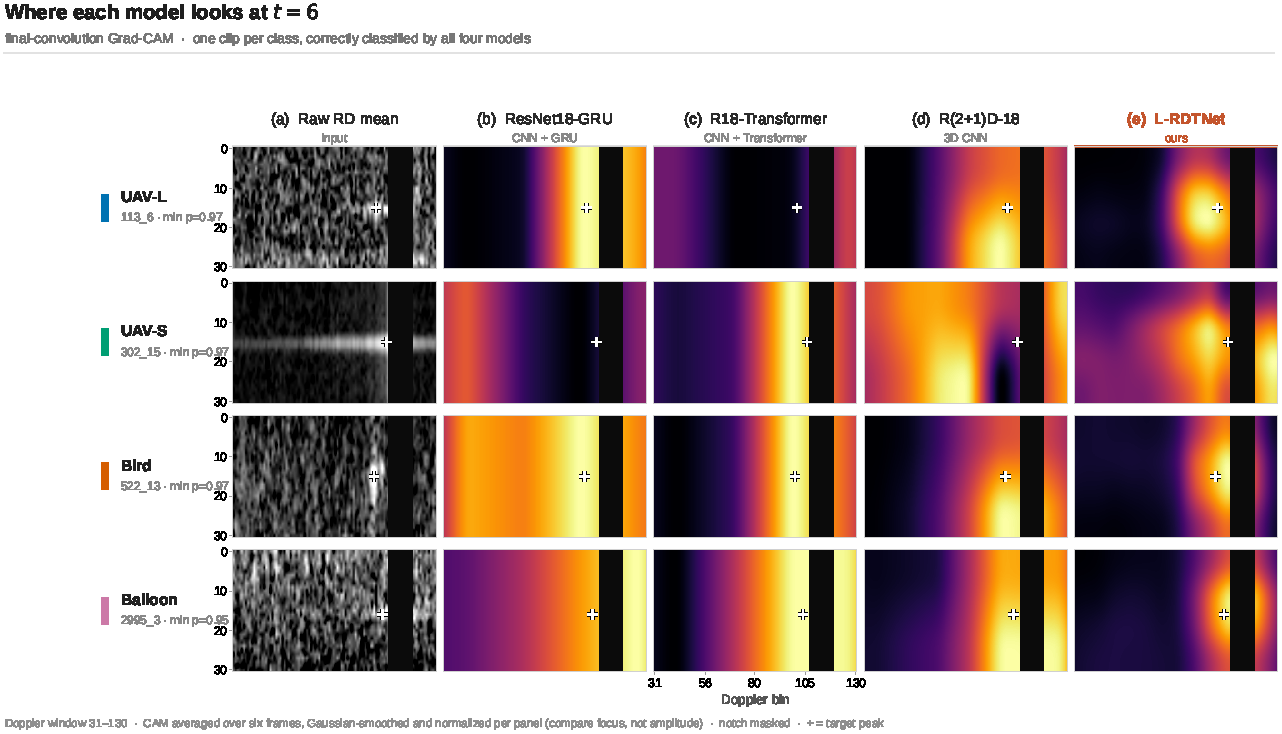
\includegraphics[width=\textwidth]{suite_model_cam_comparison.pdf}
  \caption{Where each model looks at $t=6$: final-convolution Grad-CAM of
  ResNet18-GRU, R18-Transformer, R(2+1)D-18 and L-RDTNet on one clip per class.
  All four clips are correctly classified by all four models (minimum true-class
  probability 0.949). CAMs are averaged over the six frames and normalized per
  panel, so the comparison is about spatial focus rather than amplitude. The
  baseline CNNs produce broad Doppler-band responses, while L-RDTNet is
  localized around the target peak.}
  \label{fig:model_cam_comparison}
\end{figure*}

\begin{figure*}[t]
  \centering
  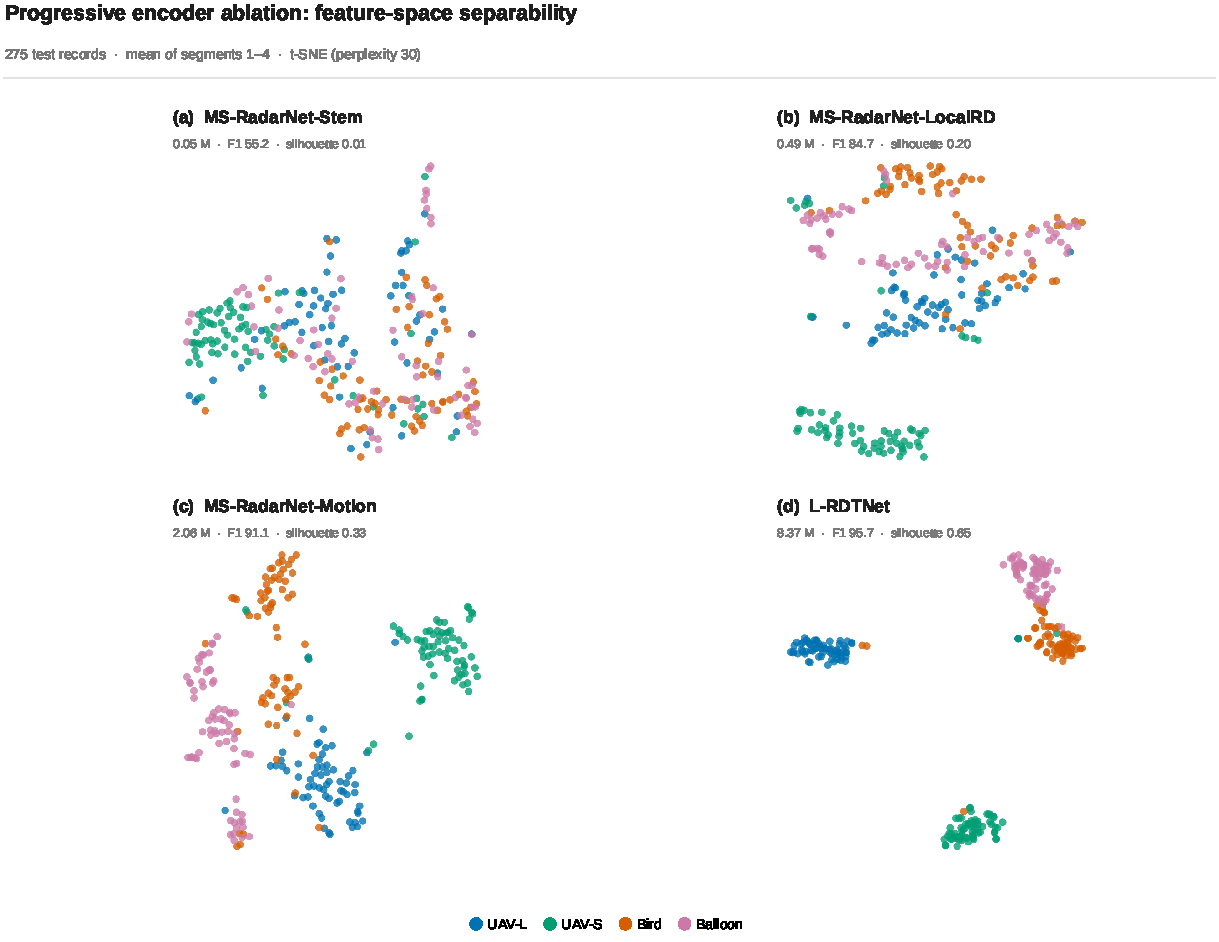
\includegraphics[width=\textwidth]{suite_ablation_tsne.pdf}
  \caption{Progressive encoder ablation in feature space. t-SNE of the 275 test
  records (features averaged over the first four segments) for
  MS-RadarNet-Stem, MS-RadarNet-LocalRD, MS-RadarNet-Motion and L-RDTNet. The
  four-class silhouette increases from 0.015 to 0.202, 0.328 and 0.653, matching
  the record-level cumulative Macro-F1 of 55.20, 84.67, 91.08 and 95.74. The
  stem features are almost inseparable, while the full encoder produces compact
  per-class clusters. Features are from the seed-42 checkpoints; the F1 values
  are the three-seed means from the ablation table.}
  \label{fig:ablation_tsne}
\end{figure*}
